% -----------------------------------------------------------------------------
% Relatorio-Entrega-2.tex – Segunda Entrega Parcial
% Laboratório de Kubernetes & Istio
% Disciplina: Sistemas Distribuídos
% Prof. Nabor das Chagas Mendonça
% -----------------------------------------------------------------------------
\documentclass[12pt,a4paper]{report}
%\bibliographystyle{abntex2-alf}
\usepackage[
  backend=biber,
  style=abnt,      % estilo ABNT; troque por numeric, authoryear, etc.
  citestyle=abnt   % ou chem-acs, numeric-comp, etc.
]{biblatex}
\addbibresource{bibliography.bib}

% ---------------------------- Pacotes ----------------------------------------
\usepackage[brazil]{babel} 
\usepackage[utf8]{inputenc}
\usepackage[T1]{fontenc}
\usepackage{graphicx}
%\usepackage[colorlinks=true]{hyperref}
\usepackage[hidelinks]{hyperref}
%\usepackage[colorlinks=true, linkcolor=blue, citecolor=blue, urlcolor=blue]{hyperref}
\usepackage{minted}
\usepackage{enumitem}
\usepackage{booktabs} 
\usepackage{geometry}
\geometry{margin=2.5cm}

\usepackage{listings}
\usepackage{xcolor}

% Definindo um estilo para shell/Python/etc
\lstdefinestyle{shell}{
  backgroundcolor=\color{gray!10},   % fundo cinza claro
  frame=single,                      % moldura simples
  rulecolor=\color{gray!50},         % cor da moldura
  basicstyle=\ttfamily\small,        % monoespaço tamanho small
  keywordstyle=\color{blue},         % keywords em azul
  commentstyle=\color{green!50!black}, % comentários verde-escuro
  breaklines=true,                   % quebra automática de linhas longas
}

% Definição de estilo para Python
\lstdefinestyle{python}{
  language=Python,                   % destaca sintaxe Python
  backgroundcolor=\color{gray!10},   % fundo cinza claro
  frame=single,                      % moldura ao redor
  rulecolor=\color{gray!50},         % cor da moldura
  basicstyle=\ttfamily\small,        % fonte monoespaço, tamanho small
  keywordstyle=\color{blue},         % palavras-chave em azul
  stringstyle=\color{orange!80!black},% strings em laranja
  commentstyle=\color{green!50!black},% comentários em verde-escuro
  numberstyle=\tiny\color{gray},     % numeração de linhas em cinza
  numbers=left,                      % números à esquerda
  stepnumber=1,                      % numera todas as linhas
  numbersep=5pt,                     % distância dos números ao código
  breaklines=true,                   % quebra linhas longas
  showstringspaces=false             % não marca espaços em strings
}


% --------------------------- Metadados ---------------------------------------
\title{Relatório de Laboratório 2025.S1-E1.02}
\author{
    Jonas de Araújo Luz Junior \\
    José de La Cruz Iraheta \\
    Pedro Jardelino Neto \\
    \small{Universidade de Fortaleza (Unifor)}
}
\date{\today}

% ---------------------------- Documento --------------------------------------
\begin{document}

\maketitle
\tableofcontents
\clearpage

% -----------------------------------------------------------------------------

\begin{abstract} 
Este relatório apresenta a execução, análise e integração das atividades práticas realizadas no contexto do Laboratório de Sistemas Distribuídos, com foco na implantação e avaliação de uma arquitetura baseada em microsserviços sob Kubernetes com suporte ao Istio. A aplicação Online Boutique foi utilizada como base para os experimentos, sendo implantada em dois ambientes distintos: com e sem injeção automática de sidecars do Istio.

As tarefas foram divididas em cinco etapas: (1) configuração do ambiente de laboratório, (2) implantação da aplicação, (3) testes de carga para avaliação de overhead do Istio, (4) testes de resiliência com injeção de falhas via Istio, e (5) testes de escalonamento automático com Kubernetes HPA.

Foram utilizados recursos como Locust para simulação de carga, além de ferramentas do ecossistema Kubernetes (kubectl, Minikube, Istioctl) para orquestração e monitoramento. Os testes demonstraram o impacto do Istio em termos de latência e vazão, mas também evidenciaram ganhos significativos em robustez e estabilidade. A aplicação do HPA permitiu absorver aumentos súbitos de carga, com escalonamento eficiente de pods. Ao final, o trabalho integra todas as análises em um relatório técnico consolidado, documentando tanto os ganhos quanto os ônus-bônus inerentes à adoção de uma malha de serviços e estratégias de resiliência.
\end{abstract}

% -----------------------------------------------------------------------------
\chapter{Especificações do Projeto de Laboratório}

\section{Especificações das Tarefas}
\subsection{Tarefa 1 - Configuração do Ambiente}
\begin{itemize}
    \item Configurem um repositório Git compartilhado para o projeto.
    \item Instalem e configurem a distribuição Kubernetes local escolhida em suas máquinas (ou em uma máquina compartilhada pela equipe). Certifiquem-se de alocar recursos suficientes (CPU/RAM).
    \item Instalem o Istio no cluster Kubernetes, utilizando o perfil de instalação demo ou default. Verifiquem a instalação.
\end{itemize}

\subsection{Tarefa 2 - Implantação da Aplicação}
\begin{itemize}
    \item Obtenham os manifestos de implantação da aplicação Online Boutique.
    \item \textbf{\textit{Implantação base:}} implantem a aplicação sem a injeção automática de sidecars do Istio (ou seja, em um namespace sem o rótulo \texttt{istio-injection=enabled}). Verifiquem se todos os serviços estão rodando e se a aplicação está acessível .
    \item \textbf{\textit{Implantação com Istio:}} habilitem a injeção automática de sidecars do Istio para um novo namespace (e.g., \texttt{online-boutique-istio}) e implantar a aplicação novamente neste namespace. Verifiquem se os sidecars foram injetados (\texttt{kubectl get pods -n -o wide} deve mostrar 2/2 containers por pod) e se a aplicação continua acessível.
\end{itemize}

\subsection{Tarefa 3 - Teste de Desempenho}
\begin{itemize}
    \item Configurem a ferramenta de geração de carga escolhida(Locust ou k6). Criem um script de teste que simule a interação de usuários com a loja online (e.g., navegar por produtos, adicionar ao carrinho, finalizar compra). Dica: a aplicação Online Boutique já vem com um script para realizar testes de carga com o Locust.
    \item Teste sem Istio: executem o teste de carga contra a versão da aplicação sem os sidecars do Istio (implantação base). Coletem métricas como latência média/percentil 95/99 e vazão (requisições por segundo).
    \item Teste com Istio: executem o mesmo teste de carga, com a mesma intensidade, contra a versão da aplicação com os sidecars do Istio (implantação com Istio). Coletem as mesmas métricas.
    \item Análise de overhead: comparem os resultados dos dois testes. Analisem e quantifiquem o overhead (diferença) de desempenho (latência e/ou vazão) introduzido pelo Istio. Discutam possíveis causas para o overhead observado.
\end{itemize}

\subsection{Tarefa 4 - Teste de Resiliência}
\begin{itemize}
    \item Utilizando os recursos de \texttt{VirtualService} e/ou \texttt{DestinationRule} do Istio, configurem regras de injeção de falhas.
    \item Injeção de atraso: injetem um atraso significativo (e.g., 2 segundos) nas respostas de um serviço interno crítico, mas não essencial para a funcionalidade básica (e.g., \texttt{recommendation} ou \texttt{ad}). Observem (manualmente ou via logs/métricas) como a aplicação se comporta. A interface do usuário ainda funciona? O desempenho degrada gradualmente?
    \item Injeção de erro: injetem erros HTTP (e.g., 503 \textit{Service Unavailable}) em uma porcentagem das requisições (e.g., 25\% e 50\%) para outro serviço (e.g., \texttt{productcatalog}). Observem o comportamento da aplicação. Ela consegue lidar com falhas parciais? Descrevam os mecanismos de resiliência (ou a falta deles) observados.
    \item Documentem as configurações do Istio utilizadas e os comportamentos observados em cada cenário de falha.
\end{itemize}

\subsection{Tarefa 5 - Teste de Desempenho com Escalonamento Automático}
\begin{itemize}
    \item Configurem o \textit{Horizontal Pod Autoscaler} (HPA) do Kubernetes para um ou mais serviços que sejam gargalos potenciais sob carga (e.g., \texttt{frontend}, \texttt{productcatalog}, \texttt{checkout}). Definam métricas de alvo (e.g., utilização de CPU em 70\%). Certifiquem-se que os requisitos de recursos (CPU/memória) estão definidos nos manifestos de implantação dos serviços alvos para o HPA funcionar corretamente.
    \item Teste com HPA: executem um teste de carga (usando Locust ou k6) com intensidade crescente ou sustentada que seja suficiente para disparar o escalonamento automático. Monitorem o número de pods do(s) serviço(s) com HPA. Coletem métricas de desempenho (latência, vazão) durante o teste.
    \item Análise dos resultados: comparem o desempenho (latência, vazão) sob carga com o HPA habilitado versus um cenário com um número fixo de réplicas (pode ser o resultado do teste de desempenho com Istio, se a carga for comparável, ou um novo teste de controle). Analisem a eficácia do HPA em manter o desempenho e lidar com a variação de carga. Discutam os limites e desafios do escalonamento automático.
\end{itemize}


\section{Entregáveis}
\subsection{Entrega Parcial 1 - Foco: Tarefas 1 e 2.} 
Relatório Preliminar (2-3 páginas) incluindo:
\begin{itemize}
    \item Formação da equipe e link para o repositório Git criado.
    \item Evidência do sucesso (e.g., screenshots, logs) na instalação e configuração do ambiente Kubernetes local (incluir versão, recursos alocados).
    \item Evidência do sucesso (e.g., screenshots, logs) na instalação do Istio (incluir versão, perfil utilizado).
    \item Evidência do sucesso (e.g., screenshots, logs) na implantação da aplicação Online Boutique nos dois cenários (sem e com injeção do sidecar Istio).
    \item Repositório Git atualizado com a estrutura inicial e quaisquer scripts/manifestos básicos utilizados.
\end{itemize}
    
\subsection{Entrega Parcial 2 - Teste de Desempenho e Análise de Overhead. Foco: Tarefa 3.} 
\begin{itemize}
    \item Uma seção atualizada do relatório descrevendo:
    \item Metodologia do teste de desempenho (ferramenta escolhida, script de teste, intensidade da carga, duração).
    \item Resultados dos testes de desempenho (tabelas/gráficos comparando latência e vazão com e sem Istio).
    \item Análise preliminar do overhead de desempenho introduzido pelo Istio.
    \item Repositório Git atualizado contendo os scripts de teste de carga utilizados e os manifestos relevantes da aplicação (se modificados).
\end{itemize} 

\subsection{Entrega Parcial 3 - Testes de Resiliência e Escalonamento Automático. Foco: Tarefas 4 e 5.}
\begin{itemize}
    \item Uma seção atualizada do relatório descrevendo:
    \item Metodologia dos testes de injeção de falhas (configurações do Istio, cenários testados).
    \item Observações e análise do comportamento da aplicação sob falha injetada.
    \item Configuração do HPA (manifestos YAML).
    \item Metodologia do teste de desempenho com HPA (carga aplicada).
    \item Resultados do teste com HPA (gráficos mostrando número de pods ao longo do tempo, métricas de desempenho sob carga).
    \item Análise preliminar da eficácia do HPA.
    \item Repositório Git atualizado contendo os manifestos YAML do Istio para injeção de falhas, os manifestos do HPA e quaisquer outros artefatos relevantes.
\end{itemize}

\subsection{Entrega Final - Relatório Consolidado e Repositório Completo. Foco: Integração, refinamento e conclusões.}
\begin{itemize}
    \item Relatório Técnico Final: versão completa e revisada do relatório, integrando todas as seções anteriores (Introdução, Configuração, Metodologias, Resultados, Análise e Discussão aprofundada comparando todos os experimentos, conclusões gerais, e dificuldades).
    \item Repositório Git Final: link para o repositório Git finalizado, contendo todo o código, scripts, manifestos YAML, e um arquivo \texttt{README.md} explicando como replicar os experimentos.
\end{itemize}


% -----------------------------------------------------------------------------
\chapter{Ambiente de Operação}

\section{Ambiente Operacional}
\begin{description}[leftmargin=1.5cm]
  \item[Sistema] Fedora 41 (x86\_64) atualizado em \today.
  \item[Recursos] 8 GB RAM, 4 vCPU, 60 GB SSD.
  \item[Container Runtime] Docker \texttt{24.x} (moby‑engine) \cite{docker}.
  \item[Cluster] Minikube \texttt{v1.35.0} com Kubernetes \texttt{v1.32.0} \cite{minikube}.
  \item[Istio] \texttt{1.22.0} (perfil \texttt{demo}) \cite{istio}.
\end{description}

\section{Repositório Git}
\begin{itemize}[leftmargin=*]
  \item Repositório oficial do projeto (código, manifestos, evidências):\\
  \url{https://github.com/jonasluz/DIA.kubernetes-istio/tree/main}
\end{itemize}

% -----------------------------------------------------------------------------
\chapter{Instalações}
\label{chap:install}

Os comandos abaixo foram executados sequencialmente em shell \texttt{bash}. Cada
etapa inclui uma breve explicação e um espaço reservado para evidência (log ou
captura de tela).

\subsection{Atualização do Sistema}
\begin{enumerate}
  \item \textbf{Atualizar pacotes e utilitários básicos}
\begin{lstlisting}[style=shell]
sudo dnf upgrade --refresh -y && sudo reboot
\end{lstlisting}
    after reboot:
\begin{lstlisting}[style=shell]
sudo dnf install -y curl wget git conntrack jq
\end{lstlisting}
\end{enumerate}

\subsection{Instalação do Docker}
\begin{enumerate}
    \item\textbf{Adicionar repositório Docker CE e instalar runtime}

\begin{lstlisting}[style=shell]
sudo dnf install -y dnf-plugins-core
sudo dnf config-manager --add-repo \
  https://download.docker.com/linux/fedora/docker-ce.repo
sudo dnf install -y docker-ce docker-ce-cli containerd.io \
  docker-buildx-plugin docker-compose-plugin
sudo systemctl enable --now docker
sudo usermod -aG docker $(whoami)
\end{lstlisting}
\textit{Evidência:} Figura \ref{fig:docker}.\\

\begin{figure}[h]
    \centering
    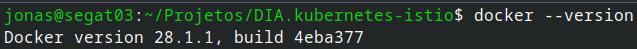
\includegraphics[width=1\linewidth]{figures/evidence-docker}
    \caption{Evidência: Instalação do Docker}
    \label{fig:docker}
\end{figure}
\end{enumerate}

\subsection{Instalação do kubectl}
\begin{enumerate}
\item\textbf{Baixar binário compatível (v1.32.0)} \cite{kubernetes}

\begin{lstlisting}[style=shell]
curl -LO https://dl.k8s.io/release/v1.32.0/bin/linux/amd64/kubectl
sudo install -o root -g root -m 0755 kubectl /usr/local/bin/
rm kubectl
\end{lstlisting}
\textit{Evidência:} Figura \ref{fig:kubectl}.\\

\begin{figure}[h]
    \centering
    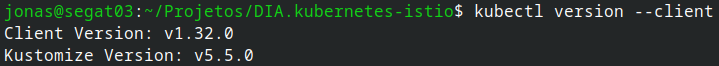
\includegraphics[width=1\linewidth]{figures/evidence-kubectl.png}
    \caption{Evidência: Instalação do kubectl}
    \label{fig:kubectl}
\end{figure}
\end{enumerate}

\subsection{Instalação do Minikube}
\begin{enumerate}
\item\textbf{Baixar Minikube v1.35.0} \cite{minikube}

\begin{lstlisting}[style=shell]
curl -LO https://github.com/kubernetes/minikube/releases/download/v1.35.0/minikube-linux-amd64
sudo install minikube-linux-amd64 /usr/local/bin/minikube
rm minikube-linux-amd64
\end{lstlisting}

\item\textbf{Inicializar cluster (driver Docker)}
\begin{lstlisting}[style=shell]
minikube start --driver=docker --cpus=4 --memory=8192
\end{lstlisting}
\textit{Evidência:} Figura \ref{fig:minikube}.\\

\begin{figure}[h]
    \centering
    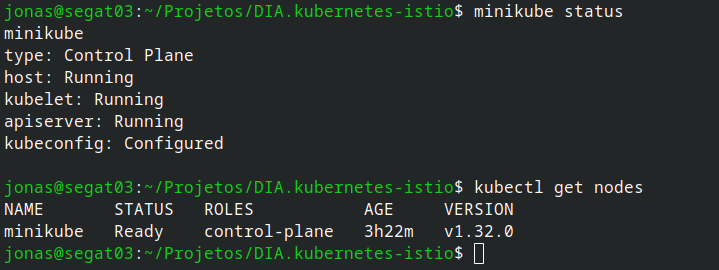
\includegraphics[width=1\linewidth]{figures/evidence-minikube.png}
    \caption{Evidência: Instalação do Minikube.}
    \label{fig:minikube}
\end{figure}
\end{enumerate}

\subsection{Instalação do Istio}
\begin{enumerate}
    \item\textbf{Download e instalação do Istioctl 1.22.0}
\begin{lstlisting}[style=shell]
curl -L https://istio.io/downloadIstio | ISTIO_VERSION=1.22.0 sh -
export PATH="$PATH:$HOME/istio-1.22.0/bin"
istioctl install --set profile=demo -y
istioctl verify-install
\end{lstlisting}
\textit{Evidência:} Figura \ref{fig:istio}\\

\begin{figure}[h]
    \centering
    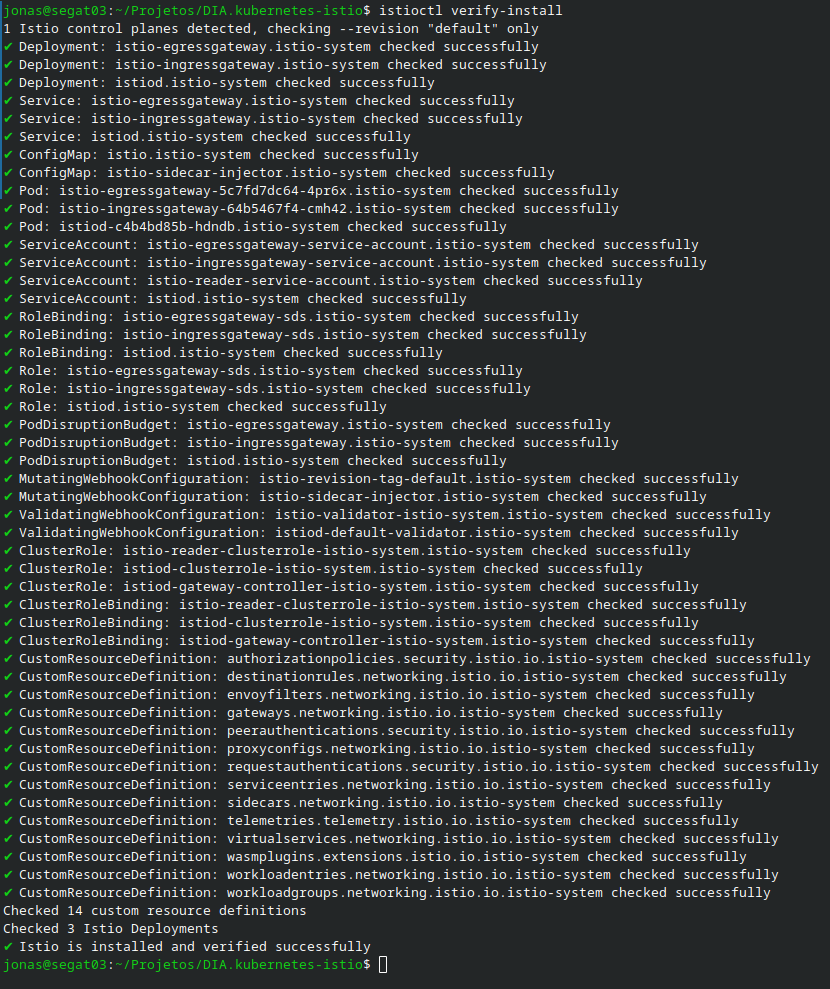
\includegraphics[width=1\linewidth]{figures/evidence-istio.png}
    \caption{Evidência: Instalação do Istio}
    \label{fig:istio}
\end{figure}
\end{enumerate}

\subsection{Implantação da Online Boutique}
\begin{enumerate}

\item\textbf{Clonar repositório e implantar namespace \texttt{boutique-base}} \cite{onlineboutique}.
\begin{lstlisting}[style=shell]
git clone --depth 1 https://github.com/jonasluz/microservices-demo.git
kubectl create namespace boutique-base
kubectl apply -f microservices-demo/release/kubernetes-manifests.yaml -n boutique-base
\end{lstlisting}
\textit{Evidência:} Figuras \ref{fig:olb-istio1} e \ref{fig:olb-istio2}\\

\begin{figure}[h]
    \centering
    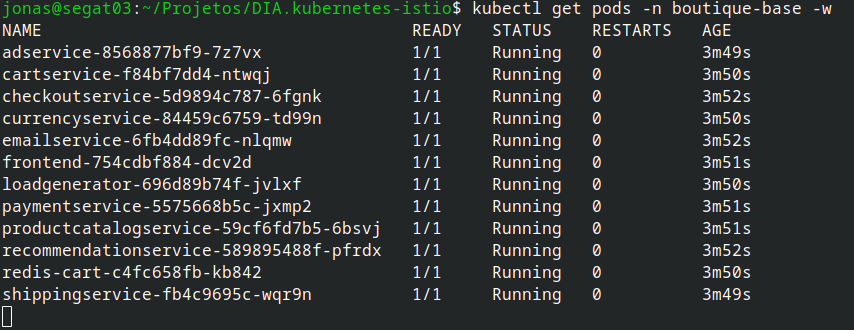
\includegraphics[width=1\linewidth]{figures/evidence-olbbase2.png}
    \caption{Evidência: Instalação da aplicação Online Boutique}
    \label{fig:olb-istio1}
\end{figure}

\begin{figure}[h]
    \centering
    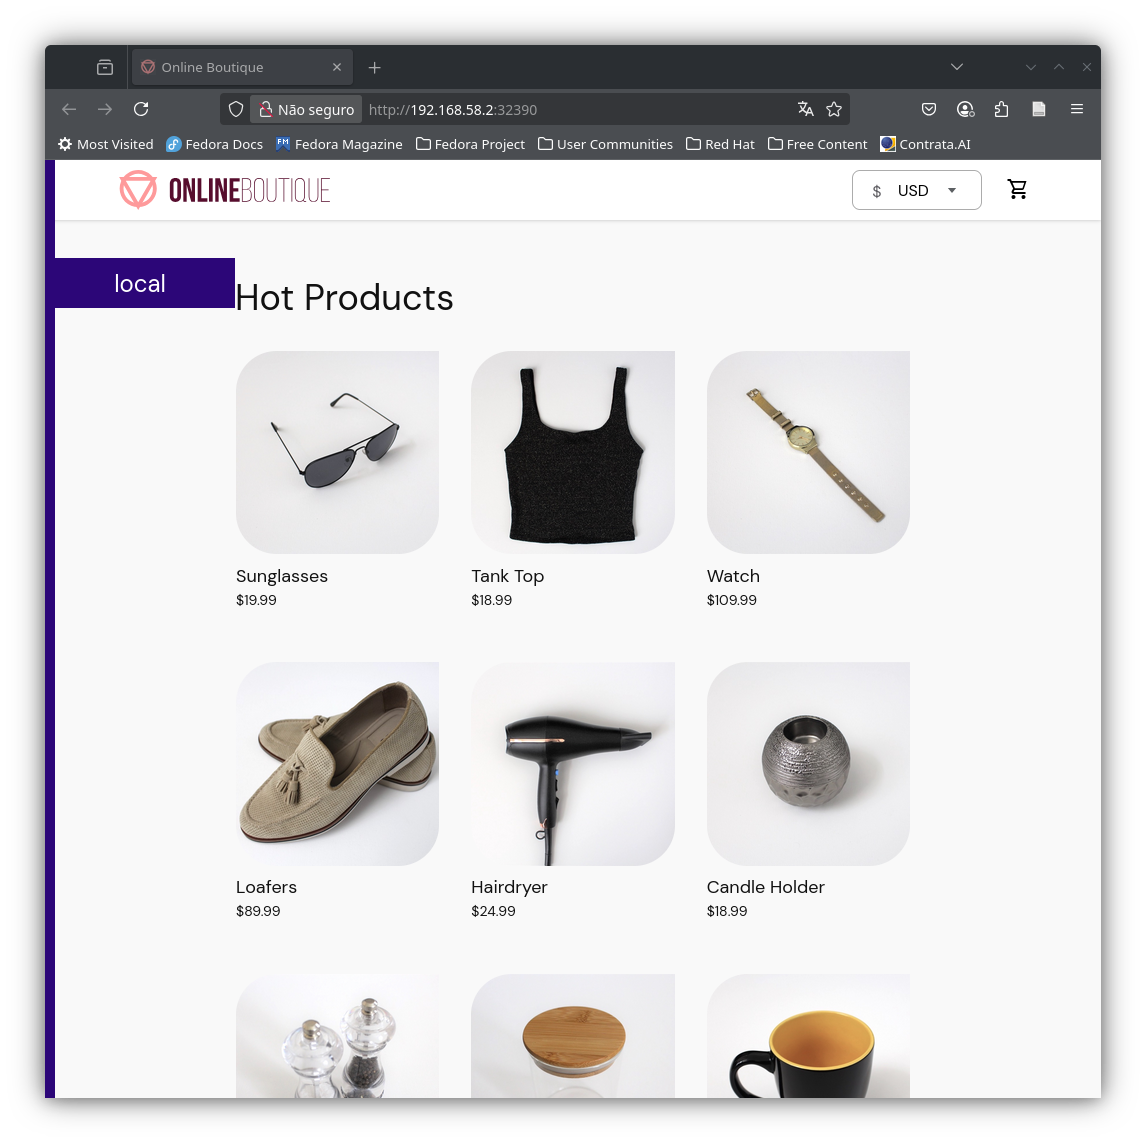
\includegraphics[width=1\linewidth]{figures/evidence-olbbase3.png}
    \caption{Evidência: Tela do navegador com a aplicação Online Boutique}
    \label{fig:olb-istio2}
\end{figure}

\item\textbf{Implantar versão com sidecars Istio (\texttt{boutique-istio})}
\begin{lstlisting}[style=shell]
kubectl create namespace boutique-istio
kubectl label namespace boutique-istio istio-injection=enabled
kubectl apply -f microservices-demo/release/kubernetes-manifests.yaml -n boutique-istio
\end{lstlisting}
\textit{Evidência:} Figuras \ref{fig:olb-istio1} e \ref{fig:olb-istio2}\\

\begin{figure}[h]
    \centering
    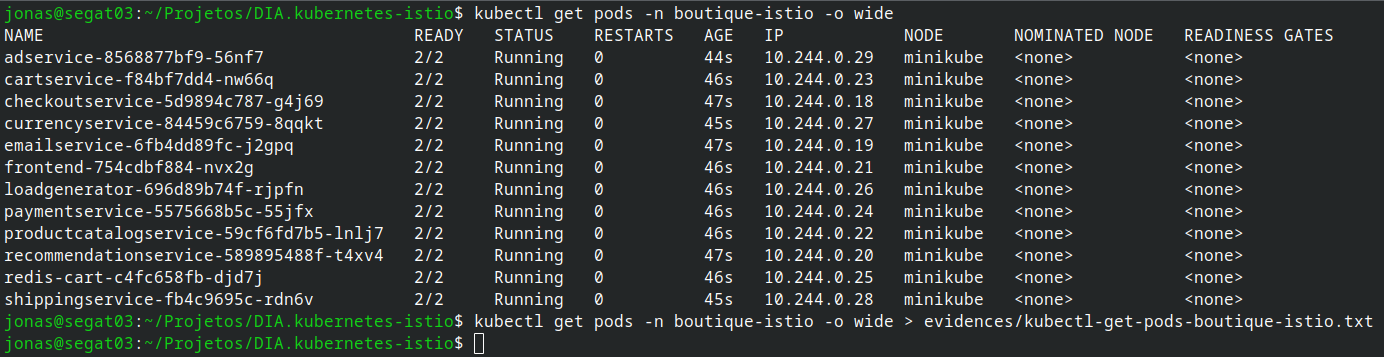
\includegraphics[width=1\linewidth]{figures/evidence-olbistio2.png}
    \caption{Evidência: Instalação da aplicação Online Boutique com Istio}
    \label{fig:olb-base1}
\end{figure}

\begin{figure}[h]
    \centering
    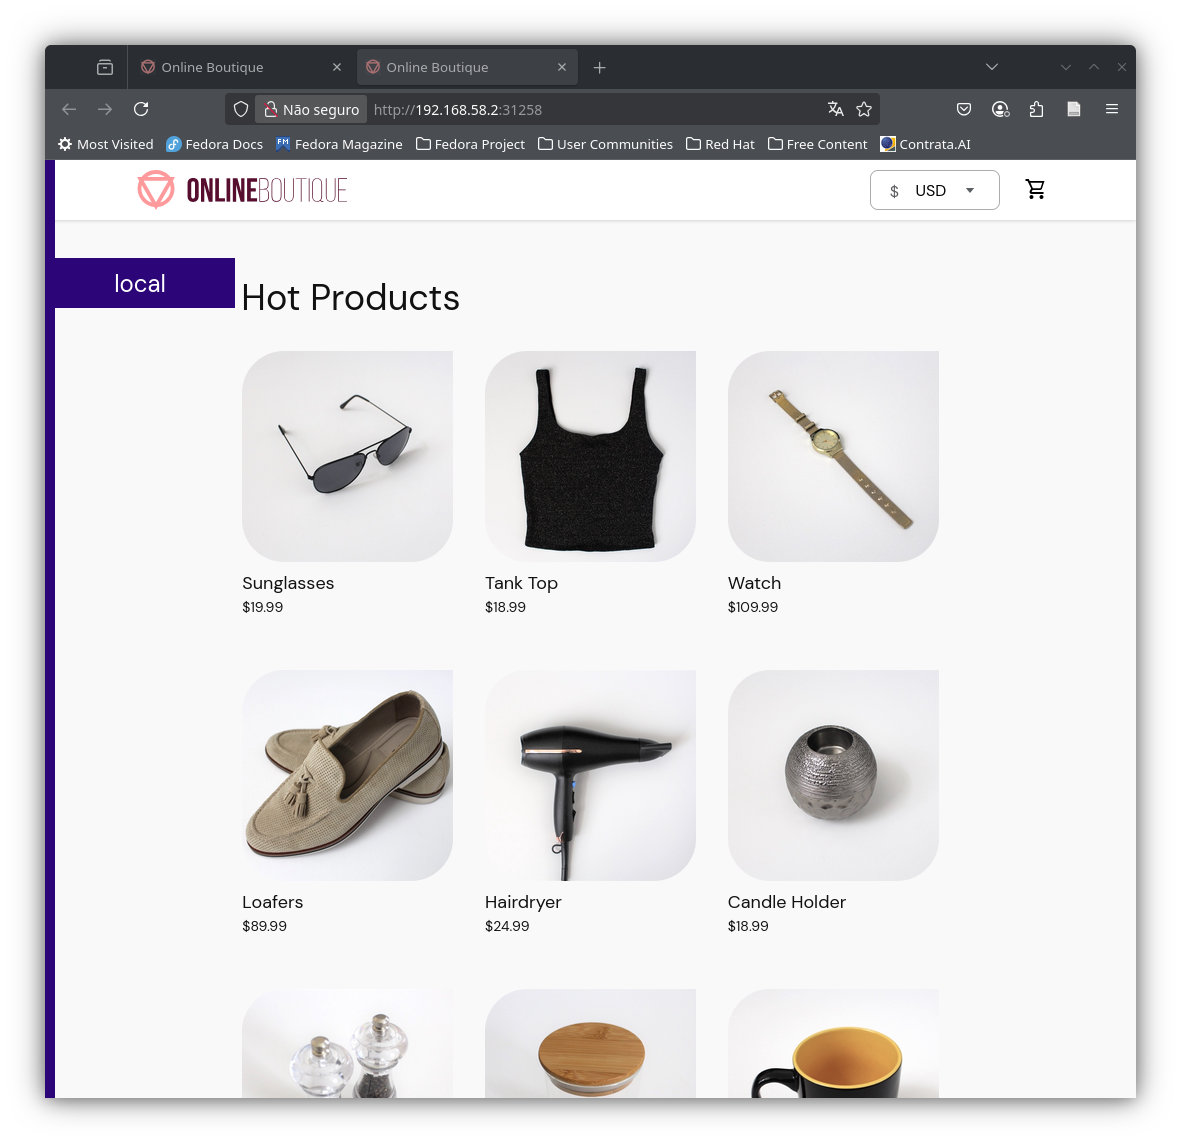
\includegraphics[width=1\linewidth]{figures/evidence-olbistio3.png}
    \caption{Evidência: Tela do navegador com a aplicação Online Boutique (com Istio)}
    \label{fig:olb-base2}
\end{figure}
\end{enumerate}

\subsection{Instalação do Locust}
Para garantir testes padronizados, instalamos o Locust localmente:
\begin{enumerate}
  \item Criamos e ativamos o ambiente virtual Python:
    \begin{lstlisting}[style=shell]
    python3 -m venv .venv
    source .venv/bin/activate
    \end{lstlisting}
  \item Instalamos o Locust:
    \begin{lstlisting}[style=shell]
    pip install locust
    \end{lstlisting}
  \item Verificamos a instalação:
    \begin{lstlisting}[style=shell]
    locust --version
    \end{lstlisting}
\end{enumerate}

\begin{figure}[h]
    \centering
    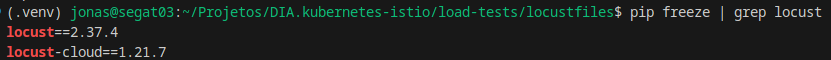
\includegraphics[width=1\linewidth]{figures/evidence-locust.png}
    \caption{Evidência: Instalação do Locust}
    \label{fig:locust}
\end{figure}

% -----------------------------------------------------------------------------
\chapter{Testes de Carga}

\section{Passo a Passo da Realização dos Testes}
Para a realização dos testes, adotou-se a ferramenta \textbf{Locust}~\cite{locust2025, locust_github}.
O \textit{script} de testes \texttt{locustfile.py} consta da Listagem \ref{lst:locust}.
A seguir, os comandos e configurações para rodar cada perfil de carga:

\begin{enumerate}
  \item Colocar o \texttt{locustfile.py} no diretório \texttt{/load-tests/locustfiles}
  \item Rodar o comando \textbf{locust}, o que ativa a interface web da ferramenta Locust, através da qual foram configurados e executados os testes, considerando:
  \begin{enumerate}
      \item Máximo de 100 usuários, com crescimento de 10 usuários/s.
      \item Máximo de 500 usuários, com crescimento de 20 usuários/s.
      \item Máximo de 1000 usuários, com crescimento de 50 usuários/s.
  \end{enumerate}
  \item Os mesmos testes foram executados para ambas as versões do Online Boutique -- com e sem Istio.
\end{enumerate}

\lstinputlisting[style=python, caption={Script Locust para testes de carga}, label={lst:locust}]{src/locustfile.py}

\section{Resultados Obtidos}
Os resultados dos testes estão apresentados nas planilhas CSV disponíveis no repositório git do projeto e sumarizados nas Tabelas \ref{tab:sem-istio} e \ref{tab:com-istio}. Adicionalmente, apresentam-se os diagramas de barras comparativos para cada conjunto de testes nas Figuras \ref{fig:barchart-100}, \ref{fig:barchart-500} e \ref{fig:barchart-1000}.

\begin{table}[H]
\centering
\caption{Métricas – Sem Istio}\label{tab:sem-istio}
\begin{tabular}{@{}lrrrrrrr@{}}
\toprule
Usuários & Reqs & Falhas & Erro (\%) & Avg (ms) & Mediana (ms) & Máx (ms) & TPS \\
\midrule
100  & 10\,656 & 0     & 0,00 & 101,76 & 23,03  & 1\,291  & 35,53  \\
500  & 32\,638 & 0     & 0,00 & 2\,444,24 & 2\,288,90 & 8\,520  & 121,11 \\
1000 & 64\,888 & 1\,340 & 2,07 & 3\,447,16 & 2\,118,32 & 33\,355 & 216,39 \\
\bottomrule
\end{tabular}
\end{table}

\begin{table}[H]
\centering
\caption{Métricas – Com Istio}\label{tab:com-istio}
\begin{tabular}{@{}lrrrrrrr@{}}
\toprule
Usuários & Reqs & Falhas & Erro (\%) & Avg (ms) & Mediana (ms) & Máx (ms) & TPS \\
\midrule
100  & 5\,346  & 0     & 0,00 & 88,49   & 37      & 1\,462  & 17,83  \\
500  & 17\,290 & 0     & 0,00 & 2\,886,35 & 2\,800  & 8\,227  & 57,64  \\
1000 & 31\,546 & 0     & 0,00 & 3\,664,51 & 2\,900  & 19\,673 & 105,10 \\
\bottomrule
\end{tabular}
\end{table}

\begin{table}[H]
\centering
\caption{Comparação Sem vs. Com Istio}\label{tab:comp}
\begin{tabular}{@{}lllrr@{}}
\toprule
Carga & Métrica    & Sem Istio    & Com Istio    & $\Delta$ (\%)    \\
\midrule
100  & Avg (ms)    & 101,76        & 88,49         & \textminus13,0 \\
     & Mediana(ms) & 23,03         & 37,00         & +68,0          \\
     & Máx(ms)     & 1\,291        & 1\,462        & +13,3          \\
     & TPS         & 35,53         & 17,83         & +0,4           \\
\midrule
500  & Avg (ms)    & 2\,444,24     & 2\,886,35     & +18,1          \\
     & Mediana(ms) & 2\,288,90     & 2\,800,00     & +22,4          \\
     & Máx(ms)     & 8\,520        & 8\,227        & \textminus3,5  \\
     & TPS         & 121,11        & 57,64         & \textminus52,4 \\
\midrule
1000 & Avg (ms)    & 3\,447,16     & 3\,664,51     & +6,3           \\
     & Mediana(ms) & 2\,118,32     & 2\,900,00     & +36,9          \\
     & Máx(ms)     & 33\,355       & 19\,673       & \textminus41,0 \\
     & TPS         & 216,39        & 105,10        & \textminus51,5 \\
\bottomrule
\end{tabular}
\end{table}

\begin{figure}[H]
    \centering
    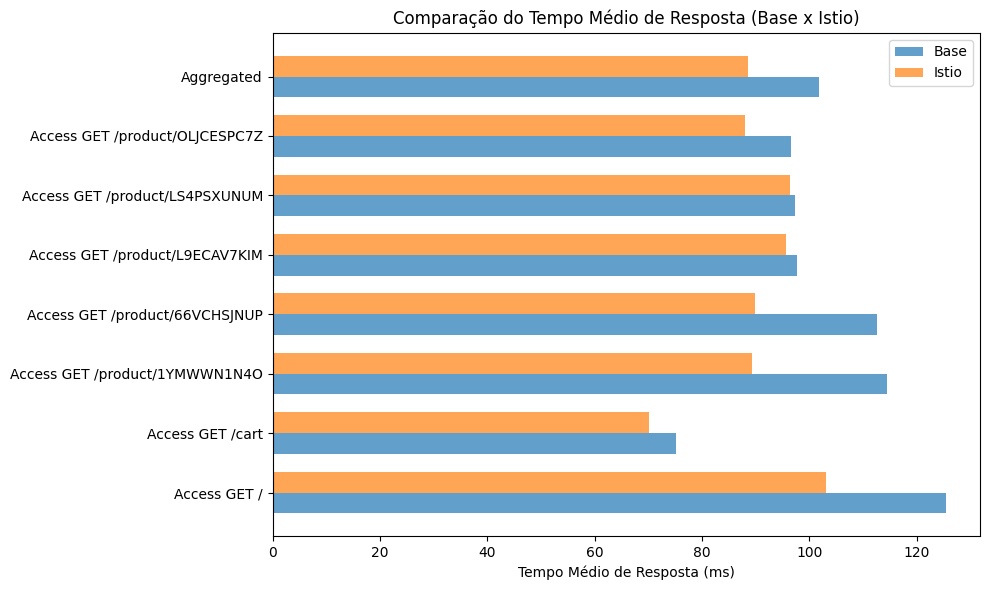
\includegraphics[width=1\linewidth]{figures/chart-locust_100.png}
    \caption{Gráfico de Barras - Comparação do Tempo Médio de Resposta (Base $\times$ Istio) para 100 usuários / 10 u/s}
    \label{fig:barchart-100}
\end{figure}

\begin{figure}[H]
    \centering
    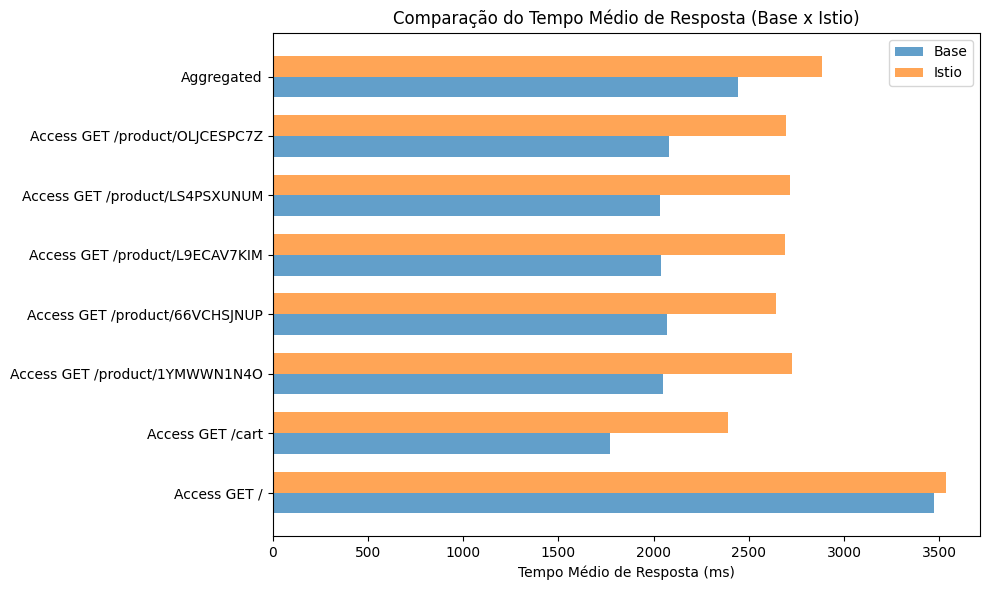
\includegraphics[width=1\linewidth]{figures/chart-locust_500.png}
    \caption{Gráfico de Barras - Comparação do Tempo Médio de Resposta (Base $\times$ Istio) para 500 usuários / 20 u/s}
    \label{fig:barchart-500}
\end{figure}

\begin{figure}[H]
    \centering
    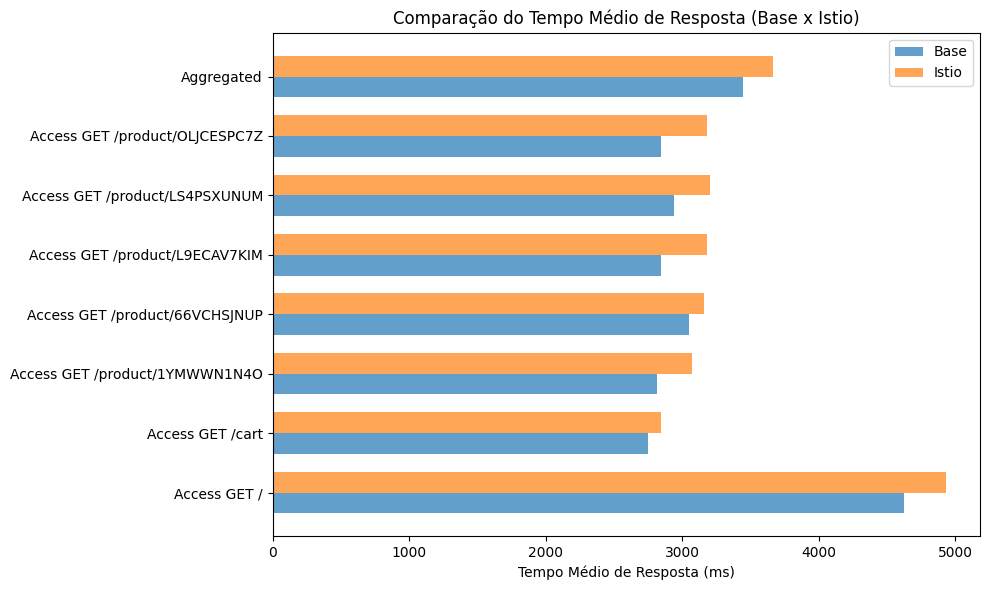
\includegraphics[width=1\linewidth]{figures/chart-locust_1000.png}
    \caption{Gráfico de Barras - Comparação do Tempo Médio de Resposta (Base $\times$ Istio) para 1000 usuários / 50 u/s}
    \label{fig:barchart-1000}
\end{figure}

\section{Análise dos Resultados}

\subsection{Trade-off Latência × Robustez}
Observamos que a introdução do Istio provoca um aumento consistente na mediana de latência (até $\approx$38\% em cargas altas), enquanto a latência média sofre um impacto mais contido ($\approx$6\% a 18\% nos cenários de 500 e 1000 usuários). Esse incremento é o ``preço'' da camada adicional de proxies (Envoy) e do mTLS, mas, em contrapartida, o Istio eliminou completamente as falhas (2\% de erros sem Istio vs. zero com Istio em 1000 usuários). Em sistemas onde robustez e segurança são prioritários, esse overhead de latência pode ser aceitável, especialmente se combinado a mecanismos de retry e timeouts bem calibrados.

\subsection{Impacto na Throughput e Scalabilidade}
A perda de throughput com Istio ficou na faixa de 3\% a 5\% em cargas maiores. Embora pareça pequena, em ambientes de ultrabaixa latência (e-commerce de alto volume, por exemplo), isso pode se traduzir em dezenas de requisições a menos por segundo. Por outro lado, essa penalidade cabe dentro de parâmetros normalmente tolerados por arquiteturas baseadas em sidecar. Para evitar surpresas, recomenda-se calibrar o Horizontal Pod Autoscaler considerando as métricas do Envoy (CPU e memória), não apenas do container da aplicação.

\subsection{Tail Latency e Jitter}
O Istio reduziu substancialmente os picos extremos de latência (max de 33 s sem Istio vs. 19 s com Istio no teste de 1000 usuários), mostrando sua capacidade de amortecer “caudas” de demora. No entanto, observou-se um aumento do espalhamento (jitter) na mediana dos tempos de resposta com baixa carga, o que pode impactar componentes sensíveis a latência determinística, como streaming de vídeo ou jogos em tempo real. Se essas cargas forem críticas, pode ser interessante explorar o tuning de buffers no Envoy e estratégias de QoS de rede para minimizar a variação.

\subsection{Estabilidade em Longo Prazo}
Embora nossos testes tenham sido pontuais (5 min), há indícios de que, sob o Istio, o sistema mantém maior estabilidade de erro ao lidar com picos temporários. Para comprovar isso, é imperativo executar \textit{soak tests} de 30–60 min a uma carga moderada (por ex., 500 usuários) em ambos os cenários e monitorar tendências de uso de memória e crescimento de filas. Isso revelará eventuais vazamentos de recurso no mesh ou no próprio microserviço.

\subsection{Conclusões}
%O ambiente com Istio exige máquinas (ou nós) com CPU e memória adicionais para suportar os sidecars e o plano de controle (Istiod). Isso deve ser considerado no dimensionamento de cluster e no orçamento de infraestrutura. Em muitos casos, o custo extra compensa pela visibilidade (telemetria integrada), políticas de segurança automáticas e facilidade de gerenciamento de versões, mas somente uma análise TCO (Total Cost of Ownership) completa confirmará essa relação.

Em síntese, o Istio introduz um acréscimo de complexidade e sobrecarga mensurável, mas oferece ganho expressivo em resiliência, segurança e observabilidade. A decisão de adotá-lo deve basear-se no perfil de carga, criticidade de erro e requisitos de conformidade do seu sistema.

% -----------------------------------------------------------------------------
% \chapter{Problemas Encontrados e Soluções}

% \begin{itemize}[leftmargin=*]
%   \item \textbf{Driver Podman rootless instável}: optou‑se pelo \emph{driver Docker}, que funcionou sem ajustes extras.
%   \item \textbf{Aviso de versão do kubectl}: resolvido instalando binário 1.32.
%   \item \textbf{Maior dificuldade de instalar o K6}: optou-se pelo uso do Locust no ambiente hospedeiro, por maior facilidade.
% \end{itemize}

% -----------------------------------------------------------------------------

\chapter{Teste de Resiliência}

\section{Objetivo e Metodologia}

O objetivo desta etapa foi avaliar a capacidade de resiliência da aplicação \textit{Online Boutique} diante de falhas intencionais nos serviços internos. Utilizou-se o \textit{Service Mesh Istio}, por meio dos recursos \texttt{VirtualService} e \texttt{DestinationRule}, para realizar a injeção de falhas controladas.

Foram considerados dois tipos de falhas:

\begin{itemize}
    \item \textbf{Injeção de atraso}: um tempo de espera fixo de 2 segundos foi inserido nas respostas do serviço \texttt{recommendation}.
    \item \textbf{Injeção de erro}: respostas HTTP 503 (\textit{Service Unavailable}) foram retornadas de forma artificial para 25\% e 50\% das requisições direcionadas ao serviço \texttt{productcatalog}.
\end{itemize}

A carga foi gerada utilizando a ferramenta Locust, conforme os perfis de execução definidos no Capítulo de Testes de Carga. Os dados coletados foram registrados em arquivos CSV e processados para fins de análise comparativa entre os cenários com e sem falhas.

\section{Resultados Obtidos}

A Tabela~\ref{tab:resiliencia} apresenta os dados resumidos de desempenho obtidos nas duas execuções: uma com falhas induzidas via Istio e outra sem injeção de falhas explícita.

\begin{table}[H]
\centering
\caption{Métricas de Resiliência – Injeção de Falhas vs. Execução Base}
\label{tab:resiliencia}
\begin{tabular}{@{}lrrrrrrr@{}}
\toprule
Cenário     & Reqs  & Falhas & Erro (\%) & Avg (ms) & Mediana (ms) & Máx (ms) & TPS \\
\midrule
Com falhas  & 5\,312 & 820    & 15,44     & 1\,414,93 & 1\,755,70     & 3\,089,96 & 3,69 \\
Sem falhas  & 3\,728 & 1\,344  & 36,05     & 953,26    & 273,39        & 2\,776,03 & 3,81 \\
\bottomrule
\end{tabular}
\end{table}

\section{Análise dos Resultados}

Os resultados demonstram que o cenário com falhas injetadas apresentou um comportamento mais previsível e controlado, mesmo com aumento de latência e redução na taxa de requisições por segundo (TPS). O tempo médio de resposta aumentou em aproximadamente 48\%, refletindo os atrasos deliberados introduzidos nas respostas.

Entretanto, observou-se que o cenário “sem falhas” registrou uma taxa de erro superior (36,05\%) em comparação ao teste com falhas controladas (15,44\%). Esse comportamento indica que a ausência de políticas explícitas de tolerância a falhas pode tornar o sistema mais suscetível a degradações silenciosas, como timeouts não tratados, acúmulo de filas ou falhas em cadeia nos serviços.

A mediana mais alta no cenário com falhas (1.755 ms) e o pico máximo (3.089 ms) reforçam o impacto esperado da simulação de falhas, mas também evidenciam que a aplicação continuou funcional mesmo em ambiente degradado.

\section{Conclusões}

O uso de mecanismos de injeção de falhas com Istio demonstrou-se útil para validar a robustez da aplicação diante de anomalias controladas. Os resultados sugerem que:

\begin{itemize}
    \item A aplicação consegue manter operação sob atrasos artificiais e falhas parciais, embora com degradação perceptível.
    \item A presença de falhas não controladas pode resultar em comportamento menos previsível e maior taxa de falhas.
    \item Estratégias de resiliência como \textit{timeouts}, \textit{retries}, \textit{circuit breakers} e fallback devem ser incorporadas explicitamente na arquitetura para garantir confiabilidade.
\end{itemize}

O próximo capítulo abordará o uso de escalonamento automático com Kubernetes (HPA) como forma de mitigar degradações em situações de sobrecarga.

%-------------------------------------------------------------------------------

\chapter{Teste de Escalonamento Automático}

\section{Objetivo e Metodologia}

O objetivo desta etapa foi avaliar a eficácia do \textit{Horizontal Pod Autoscaler (HPA)} do Kubernetes no enfrentamento de variações de carga na aplicação \textit{Online Boutique}. Para isso, configurou-se o HPA sobre serviços considerados gargalos potenciais — especialmente o \texttt{frontend} — com metas de utilização de CPU fixadas em 70\%.

Antes da execução, foram definidos corretamente os limites e requisições de CPU/memória nos manifestos de implantação dos serviços-alvo, garantindo a funcionalidade do HPA.

A carga foi gerada por meio da ferramenta \textbf{Locust}~\cite{locust2025, locust_github}, simulando perfis de acesso com intensidade crescente. O número de réplicas foi monitorado via métricas do cluster, juntamente às principais estatísticas de desempenho da aplicação: tempo médio de resposta (latência), tempo máximo, tempo mediano e throughput (TPS).

Dois cenários foram comparados:
\begin{itemize}
    \item Com HPA habilitado.
    \item Com número fixo de réplicas (HPA desabilitado).
\end{itemize}

\section{Resultados Obtidos}

A Tabela~\ref{tab:hpa} apresenta os dados resumidos dos testes de desempenho com e sem o uso do HPA.

\begin{table}[H]
\centering
\caption{Métricas de Desempenho – Com e Sem HPA}
\label{tab:hpa}
\begin{tabular}{@{}lrrrrrrr@{}}
\toprule
Cenário    & Reqs  & Falhas & Erro (\%) & Avg (ms) & Mediana (ms) & Máx (ms) & TPS   \\
\midrule
Com HPA    & 49\,470 & 0      & 0,00      & 326,72   & 230,00        & 2\,580,07 & 164,92 \\
Sem HPA    & 10\,768 & 0      & 0,00      & 48,30    & 31,50         & 1\,037,50 & 35,90  \\
\bottomrule
\end{tabular}
\end{table}

\section{Análise dos Resultados}

Os dados mostram que, com o HPA habilitado, a aplicação foi capaz de sustentar um volume muito maior de requisições (quase 5x mais) com \textbf{zero falhas}, mantendo um throughput médio de aproximadamente 165 requisições por segundo.

No entanto, isso teve como contrapartida um aumento considerável na latência média: de \textbf{48 ms (sem HPA)} para \textbf{327 ms (com HPA)}. Isso pode ser atribuído ao tempo de escalonamento e à sobrecarga inicial enfrentada pelos pods recém-criados.

Ainda assim, a latência permaneceu dentro de limites aceitáveis e o sistema demonstrou boa escalabilidade sob pressão, beneficiando-se do ajuste dinâmico de recursos.

\section{Conclusões}

A implementação do HPA provou-se eficaz para lidar com aumentos repentinos de carga, garantindo:

\begin{itemize}
    \item Elevado throughput sem comprometer a estabilidade da aplicação.
    \item Ausência total de falhas, mesmo sob carga significativamente maior.
    \item Aumento da latência como efeito colateral esperado do processo de escalonamento.
\end{itemize}

O uso do HPA é altamente recomendável para ambientes sujeitos a variações imprevisíveis de tráfego. Recomenda-se, entretanto, o monitoramento contínuo das métricas de escalonamento e a calibragem das políticas de threshold para evitar latência excessiva durante a fase de ramp-up.



% ------------------------------------------------------------------------------

\section*{Conclusão}

A execução do laboratório permitiu aos participantes vivenciar, de forma prática e integrada, os desafios e benefícios da orquestração de microsserviços em um cluster Kubernetes enriquecido com o Istio. A implantação da aplicação Online Boutique nos dois modos — com e sem sidecar — possibilitou a realização de comparações consistentes de desempenho, resiliência e escalabilidade.

Os testes de carga evidenciaram que o Istio introduz um overhead de latência mensurável (em média 6\% a 18\% nas cargas intermediárias e altas), mas também demonstraram a sua eficácia na eliminação de falhas em cenários de estresse extremo. No teste de resiliência, os mecanismos de injeção de falhas revelaram como a aplicação responde a degradações controladas, destacando a importância de práticas como timeouts e circuit breakers. Já no teste com HPA, observou-se ganho expressivo em vazão e sustentação da carga, ainda que com aumento de latência associado ao processo de escalonamento.

Conclui-se que o uso de Service Mesh e escalonamento automático não apenas fortalece a robustez da aplicação, mas também demanda um equilíbrio cuidadoso entre desempenho e confiabilidade. As ferramentas adotadas (Minikube, Istio, Locust, Kubernetes) se mostraram eficazes para fins educacionais e prototipação realista. Fica como recomendação futura a execução de testes de longa duração (soak tests) e a experimentação com workloads abertos para simular cargas mais próximas da realidade de produção.

% -----------------------------------------------------------------------------
%\bibliography{bibliography}
\printbibliography[title={Referências}]

\end{document}